\documentclass[17pt]{beamer}
\usepackage[T1]{fontenc}
\usepackage[utf8]{inputenc}
\usepackage{graphicx}
\usetheme{Madrid}
\usecolortheme{beaver}
 
%Information to be included in the title page:
\title{Wstęp do uczenia maszynowego}
\subtitle{Regresja liniowa}
\author{Tomasz Derek}
\institute{KMS}
\date{Październik 23, 2019}
 
\begin{document}
 
\frame{\titlepage}
 
\begin{frame}
\frametitle{Typy uczenia}
\begin{itemize}
\item Uczenie nadzorowane
\item Uczenie nienadzorowane
\item Ucznenie przez wzmacnianie
\end{itemize}
\end{frame} 
 
\begin{frame}
\frametitle{Typy uczenia}
\begin{figure}[ht]
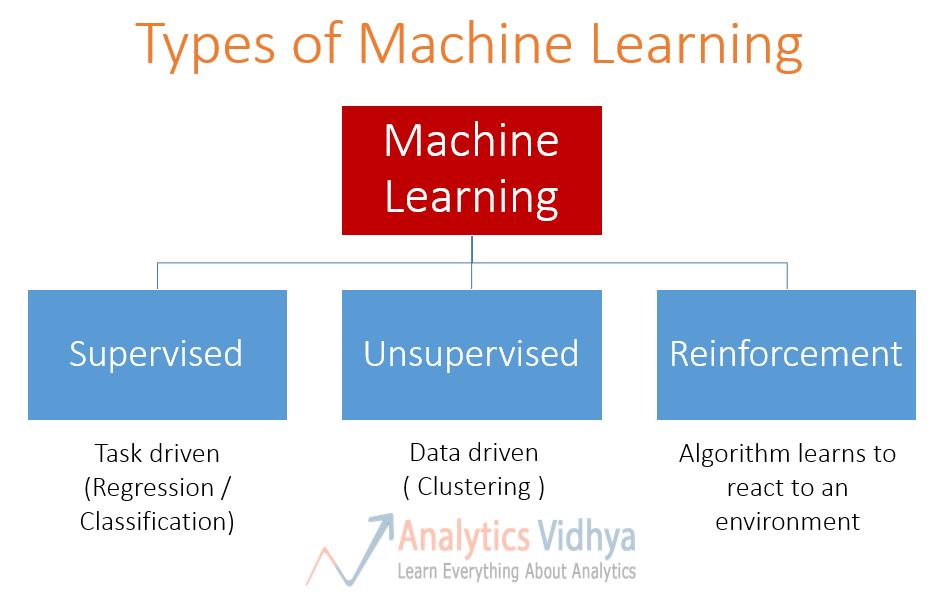
\includegraphics[scale=0.25]{./ml_types.png}
\end{figure}
\end{frame}

\end{document}https://github.com/HyperScypion/KMS_Neural_Networks/tree/master/lectures/third_lecture/notebooks